%----------------------------------------------------------------------------------------
%	PACKAGES AND OTHER DOCUMENT CONFIGURATIONS
%----------------------------------------------------------------------------------------

\documentclass[11pt,notitlepage]{article}
\usepackage{palatino} % Palatino font
\usepackage{helvet} % Helvetica font
\renewcommand*\familydefault{\sfdefault} % Use the sans serif version of the font
\usepackage[T1]{fontenc}
\linespread{1.05} % A little extra line spread is better for the Palatino font
\usepackage{lipsum} % Used for inserting dummy 'Lorem ipsum' text into the template
\usepackage{amsfonts, amsmath, amsthm, amssymb} % For math fonts, symbols and environments
\usepackage{graphicx} % Required for including images
\usepackage{booktabs} % Top and bottom rules for table
\usepackage{wrapfig} % Allows in-line images
\usepackage[labelfont=bf]{caption} % Make figure numbering in captions bold
\usepackage[top=0.5in,bottom=0.5in,left=0.5in,right=0.5in]{geometry} % Reduce the size of the margin
\pagestyle{empty} % Remove page numbers
\hyphenation{ionto-pho-re-tic iso-tro-pic fortran} % Specifies custom hyphenation points for words or words that shouldn't be hyphenated at all

\title{Permutation-based Control of False Discovery Rate}
\date{May 5, 2015}
\author{Alan Cowen \and Ye Xia \and Chris Gagne}



\begin{document}

\maketitle




%----------------------------------------------------------------------------------------
%	ABSTRACT
%----------------------------------------------------------------------------------------

\section*{Abstract}

Statistical analysis of fMRI data typically proceeds by conducting hypothesis tests on individual voxels in cortex (around 50,000), making the question of assessing statistical significance among multiple tests particularly important. Controlling the false discovery rate (FDR) is one approach to assessing statistical significance that is often used in fMRI data. However if the individual tests are correlated, the standard methods for implementing this control can yield highly variable results. By using a permutation-based method for controlling the FDR, we achieve not only control, but also an estimate of its variability. In part I, we verify the validity of the permutation-based method using simulations. In part II, we apply it to an fMRI dataset currently under analysis. In part III, in order to test the method's performance with independent tests, we apply it to an online behavioral experiment dataset.


%----------------------------------------------------------------------------------------
%	BACKGROUND
%----------------------------------------------------------------------------------------


\section*{Background}

fMRI research often seeks to map out the locations of brain regions sensitive to information about a stimulus (e.g. whether it is a face or scene), or test different models of information processing within a single region.  In doing so, many fMRI analyses follow a basic template: first, experimenters hypothesize about the stimulus features that might be important; then, they fit linear models in which the recorded brain-signal time-series is treated as a linear combination of these stimulus features plus additive noise. They then draw scientific conclusions by testing the significance of the linear models or the coefficients therein. In a typical fMRI experiment, experimenters fit linear models to each individual voxel in the recorded images, yielding around 50,000 models. Reaching decisions about statistical significance in the context of this many hypothesis tests is a relatively modern statistical challenge.

The most common solution is to extend the single hypothesis p-value, which is the probability of a type I error (i.e. false discovery), to the whole family of tests. This is known as family-wise-error rate, and it is the probability that there is at least one type I error in the entire family of tests. If V denotes the number of type I errors, FWER=Pr(V>=1). However, FWER is often considered too strict for scientific decision making. For example, if an experimenter keeps the probability of even one false discovery to 0.05, he may be ignoring many true discoveries in the experiment. (e.g he will have lower power). 

Therefore, many experimenters prefer to use the False-Discovery Rate (FDR) for deciding statistical significance. FDR is defined as the expected proportion of type I errors (V) in the set of tests declared significant, (R): FDR = E[V/R]. If the experiment were repeated many times, the experimenter would expect this proportion of the tests, on average, to be falsely declared significant each time. Benjamini and Hochberg (1995) (BH) were the first to provide an algorithm to control this quantity, which adjusts the significance threshold for p-values so that the FDR is guaranteed to be below some desired value q. For example, if we choose q=0.05, BH determines the p-value significance threshold, so that upon repeated experimentation there would be no more than 5 percent of false discoveries within our significant set. 




Although BH's guarantee for control works under minimal assumptions, it can exhibit undesirable properties when the multiple hypothesis tests are strongly correlated. It still guarantees that the proportion of false discoveries is below the desired level q in expectation; however, the actual proportion of false discoveries might fluctuate greatly across experiments. 

\begin{wrapfigure}{r}{11cm} % Example figure with text wrapping around it
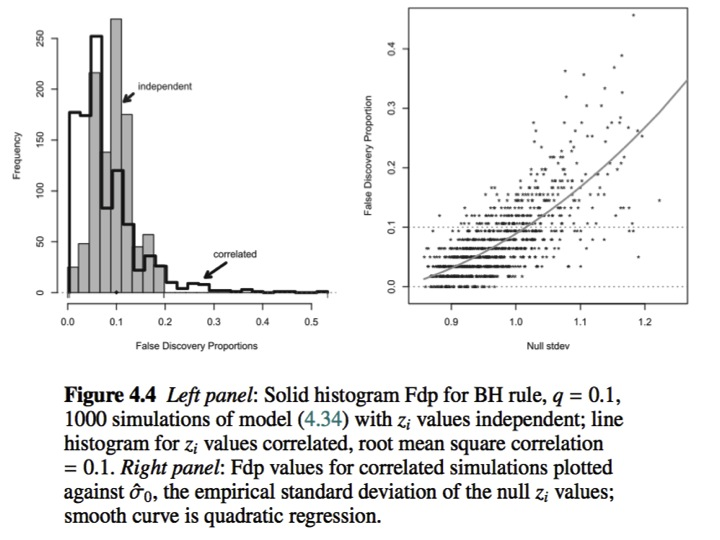
\includegraphics[scale=0.45]{Figures/Slide1.jpg}
\caption{\footnotesize Correlated hypothesis tests lead to highly variable false discovery proportions}
\end{wrapfigure}


Efron (2010) simulates this scenario (Figure 1), showing that the FDR can vary from 0 to ~40 percent when q is held at only 10 percent. Unfortunately, fMRI voxels, and thus tests, are often highly correlated. In effect, the actual proportion of false discoveries in a dataset might vary as much as in these simulations, making BH's control potentially problematic for fMRI. 




\subsection*{A permutation-based FDR control algorithm}

Is there a way to check how variable the proportion of false discoveries might be in a given fMRI dataset? Permutation of the data provides one answer to this question, as it can generate an empirical null distribution of p-values which reflects this variability. To start, we might assume as a null that the time series in a particular voxel would be exactly the same had we done our experiment in a different way. In other words, the presentation of stimuli occurring during the experiment had no effect on this particular voxel's activity. Under this assumption, we generate numerous repeats of the experiment via permutation of the design matrix and calculate the p-values obtained by the same analysis each time. We can therefore generate a joint empirical distribution of p-values across voxels for the multiple tests and repeats of the experiment. With this distribution, we can count the number tests we would have declared significant for each permutation, given a fixed p-value threshold. The sum is an estimate of the expected number of false discoveries corresponding to that threshold, because there are no true discoveries in our empirical null. We can take the mean number of tests we would have declared significant across permutations to get an unbiased estimate of expected number of false discoveries. If we divide this by the number of tests we'd declared significant in our actual results, we arrive at an estimate of FDR. Like BH, we can choose a significance threshold so that our FDR is below our desired q-level. 

So far we have just achieved the same control as BH. However, we can use our empirical null distribution to go further and estimate a confidence interval for the FDR for our dataset. If permutation is performed on the design matrix (our X), but fixed across voxels (our Y), the correlation structure across voxels is preserved and the null distribution for our FDR estimate will reflect this. Therefore, if we count the number of voxels that exceed our significance threshold in each individual permutation, this forms an empirical distribution for the number of false discoveries in our data, \textit{conditioned on the correlation structure of the voxels}. These numbers can further be divided by the number of tests we'd declared significant in our actual results, forming an empirical distribution for our FDR. The 5th and 95th percentiles of this distribution form a 90 percent confidence interval for our FDR. Furthermore, we can choose separate thresholds such that (a) in 5 percent of permutations, the estimated FDR was below q--resulting in a liberal threshold; or (b) in 95 percent of permutations, the estimated FDR was below q--resulting in a conservative threshold. Now, we can conclude that there is a 90 percent chance that the threshold we ought to be using to ensure our FDR is below q is somewhere between the liberal and the conservative thresholds--in other words, these form 90 percent confidence interval bounds for our FDR threshold. Crucially, we can look at the significance maps generated by using the liberal vs. conservative thresholds to see how much faith we should put into our FDR estimate. In essence, we get a sense of experimental repeatability, which is extremely useful for scientific decision making.


\newpage

%----------------------------------------------------------------------------------------
%	PART I: 
%----------------------------------------------------------------------------------------

\section*{Part 1: Simulations}

We conducted simulations for two purposes: (1) to demonstrate that BH control of FDR in a somewhat realistic fMRI dataset can suffer from high variability, and (2) demonstrate how permutation-based FDR control can provide an accurate estimate of this variability. To demonstrate the problem of variability, we generated 1000 datasets with high correlation across tests and compared the results to 1000 datasets with low correlation across tests. Since hypothesis tests were done on individual voxels, test correlation was implemented by adding either a high or low amount of spatially correlated noise to the simulated fMRI data. Crucially, simulation allow for the true number of false discoveries to be known, so for each dataset we can calculate a true proportion of false discoveries and see how this compares to both of our FDR estimates.

To keep the analysis simple, we used a basic (yet fairly typical) fMRI experimental design. Pictures of faces and houses were hypothetically displayed to the subject while BOLD signal was measured in a set 900 voxels, each having 400 time points of recorded activity. Voxels were responsive to faces, houses, or neither. If a voxel was responsive to an image, its activity increased from 0 to 1 during the image presentation. Otherwise, each voxel's activity fluctuated around 0 with Gaussian noise. Additional spatial noise was added to all voxels in the form of a Gaussian random field using the R-package (neuRosim). Figure 2 demonstrates the method for dataset construction. The left panel depicts two regions (red circles) that are face (left) or house (right) responsive. Their response signal to face and house images is plotted below. The middle panel depicts temporal noise and the two types of spatial noise added. The right panel depicts a temporally averaged view of the final dataset. 


\begin{figure}[h c] % Centered big figure at bottom of the page ([b] argument, could be "t" for top or "h" for here)
\centering
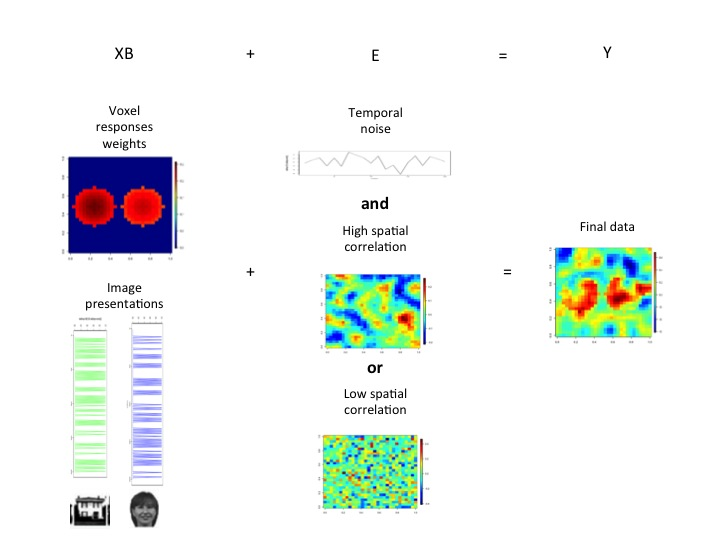
\includegraphics[scale = .60]{Figures/Slide2.jpg}
\caption{\footnotesize Method for simulating data}
\end{figure}


The hypothetical aim of this data is to assess which voxels have significant responses to face and/or houses. Therefore, for each simulation, a linear model was fit to each voxel using, as predictors, indicator variables for the presentation times of faces and houses. P-values were calculated for each of the two coefficients for each voxel, and then we used both BH as well as our permutation-based method to adjust the significance level for all voxels so that our estimated FDR<0.1. Finally, since the data was simulated, the true false discovery rate was calculated. An example simulation is depicted in Figure 3-B. The voxels that were truly responsive to faces or houses are labeled "Simulated truth," under which the voxels declared significant via BH for this simulation (under high and low spatial correlations) are labeled "Significant voxels." Many of the truly responsive voxels are declared significant, but there are also a few false discoveries outside the two regions. 

To replicate the simulation of Efron (2010), we plotted a histogram of the true number of false discoveries across all the simulations under the high-spatial correlation and low-spatial correlation conditions (Figure 3-A). The mean of both distributions was below 0.1, our desired threshold. As in Efron (2010), the high-spatial correlation condition had a much wider distribution; this held true for both the BH and permutation-based methods. On some of the simulations, the actual false discovery rate was greater than 30 percent, much higher than our desired level of 10 percent. 

The permutation-based FDR method yielded similar distributions for true false discovery rates. However, it also provided 90-percent confidence interval bounds for our false discovery rate threshold on each simulation. One example, from the high-spatial correlation condition, is shown in Figure 3-C. The middle panel depicts the mean number of voxels declared significant at q=0.1. The left and right panels depict bounds for a 90 percent confidence interval on our estimated FDR threshold. If this had been our actual dataset for an experiment, these confidence interval maps would give us a sense of how the number of significantly declared voxels might change with a repeated experiment. Here, they change quite significantly. And, since this is a simulation, we can verify that our bounds "worked": as it turns out, the threshold that would truly have yielded a 10 percent false discovery proportion lied between our confidence bounds 94 percent of the time. 


\begin{figure}[h c] % Centered big figure at bottom of the page ([b] argument, could be "t" for top or "h" for here)
\centering
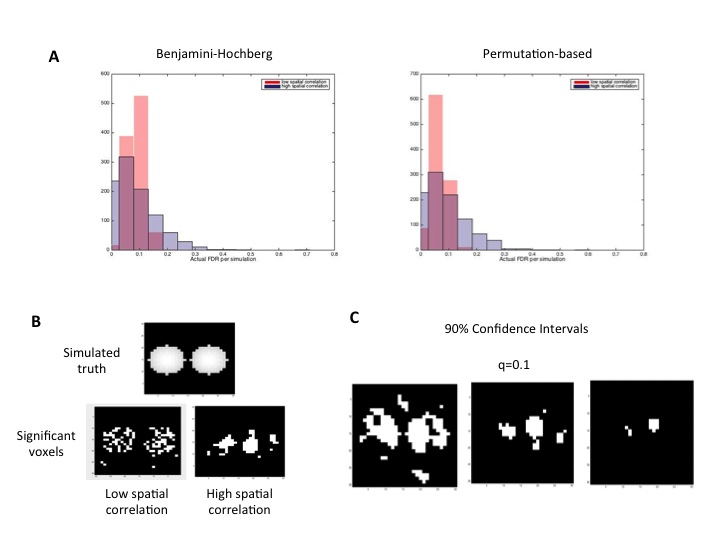
\includegraphics[scale = .60]{Figures/Slide3.jpg}
\caption{\footnotesize Simulation results}
\end{figure}



\newpage

\section*{Part 2: fMRI Dataset}


Face perception is essential to human social interactions on a daily
basis. It enables us to identify a virtually unlimited number of people,
interpret a wide range of facial emotional cues, and draw rapid trait
inferences from facial appearance. These abilities are made possible by
a network of brain regions that seem to be largely dedicated to face
perception, including the fusiform face area (FFA), occipital face area
(OFA), and posterior superior temporal sulcus (pSTS).

While it is well understood that these brain regions activate in
response to face images, it is less clear what aspects of face
processing they each perform. Our approach is to measure brain activity
in response to a large set of naturalistic faces, then use
L2-regularized regression to see if we can predict brain activity as a
function of different features of the images. Figure 1 shows how this
works.

In general, we can compare the ability of different feature models to
predict voxels in different regions across cortex. Here, for simplicity,
we use only a semantic model. Membership of each face image in 102
semantic categories was independently determined by five naive raters
and then averaged. 53 terms described variant facial attributes
including 10 aspects of facial posture (e.g.~mouth open, squinting) and
43 emotional expressions. The other 49 terms described invariant facial
attributes such as gender and race.


\begin{figure}[h c] % Centered big figure at bottom of the page ([b] argument, could be "t" for top or "h" for here)
\centering
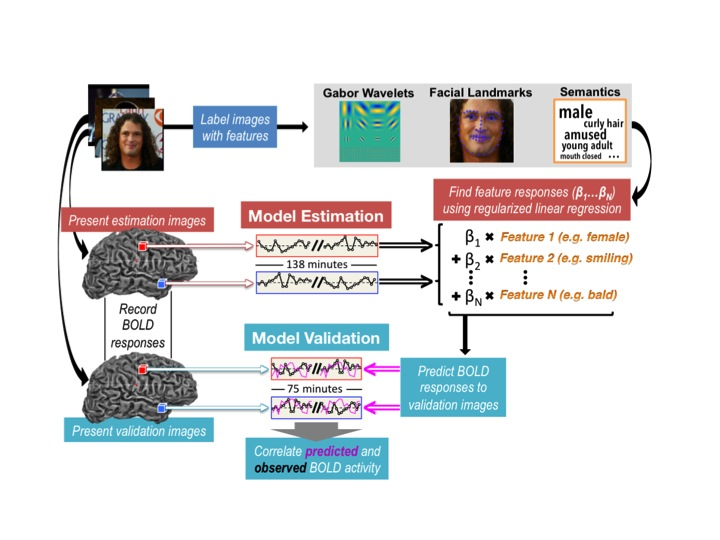
\includegraphics[scale = .60]{Figures/Slide4.jpg}
\caption{\footnotesize Method for fMRI analysis}
\end{figure}



The model was fit separately to the 1.92 hours of estimation data
collected within each individual voxel. To model the slow hemodynamic
response, variables within each model were assigned distinct
time-inseparable finite impulse response filters with four bins at
delays 2-4 s, 4-6 s, 6-8 s, and 8-10 s after stimulus onset. All model
parameters were simultaneously fit using L2-regularized linear
regression. The regularization parameter (λ) for regression was selected
with nine-fold cross-validation. Each voxel's prediction scores were
taken as the correlation coefficient (Pearson's r) between the actual
and predicted BOLD responses for that voxel. The optimal λ for all
voxels was determined by testing ten values and selecting the one for
which the maximum number of voxels had prediction scores exceeding a
threshold r value (0.06). The model-fitting procedures were performed
with in-house software written in Matlab (MathWorks). After fitting each
voxel-wise encoding model, the proportion of variance explained in each
voxel was estimated by predicting the BOLD responses to the validation
set and correlating these predictions with the data. (Figure 4). 

We test which of this correlations are significant to see which voxels behave in accordance with the encoding model. This is where we must apply FDR control. The results of applying BH and permutation-based FDR control are shown in Figure 5. 

As shown in Figure 5, the thresholds estimated by BH and permutation-based FDR control are quite similar. Notably, the 5 and 95 percent confidence bounds on the permutation-based threshold do not result in much variability in selected voxels. This suggests that correlation between voxels did not pose too much of a problem for estimating FDR, and, if the experiment were performed again, we would obtain similar results. 

\begin{figure}[h c] % Centered big figure at bottom of the page ([b] argument, could be "t" for top or "h" for here)
\centering
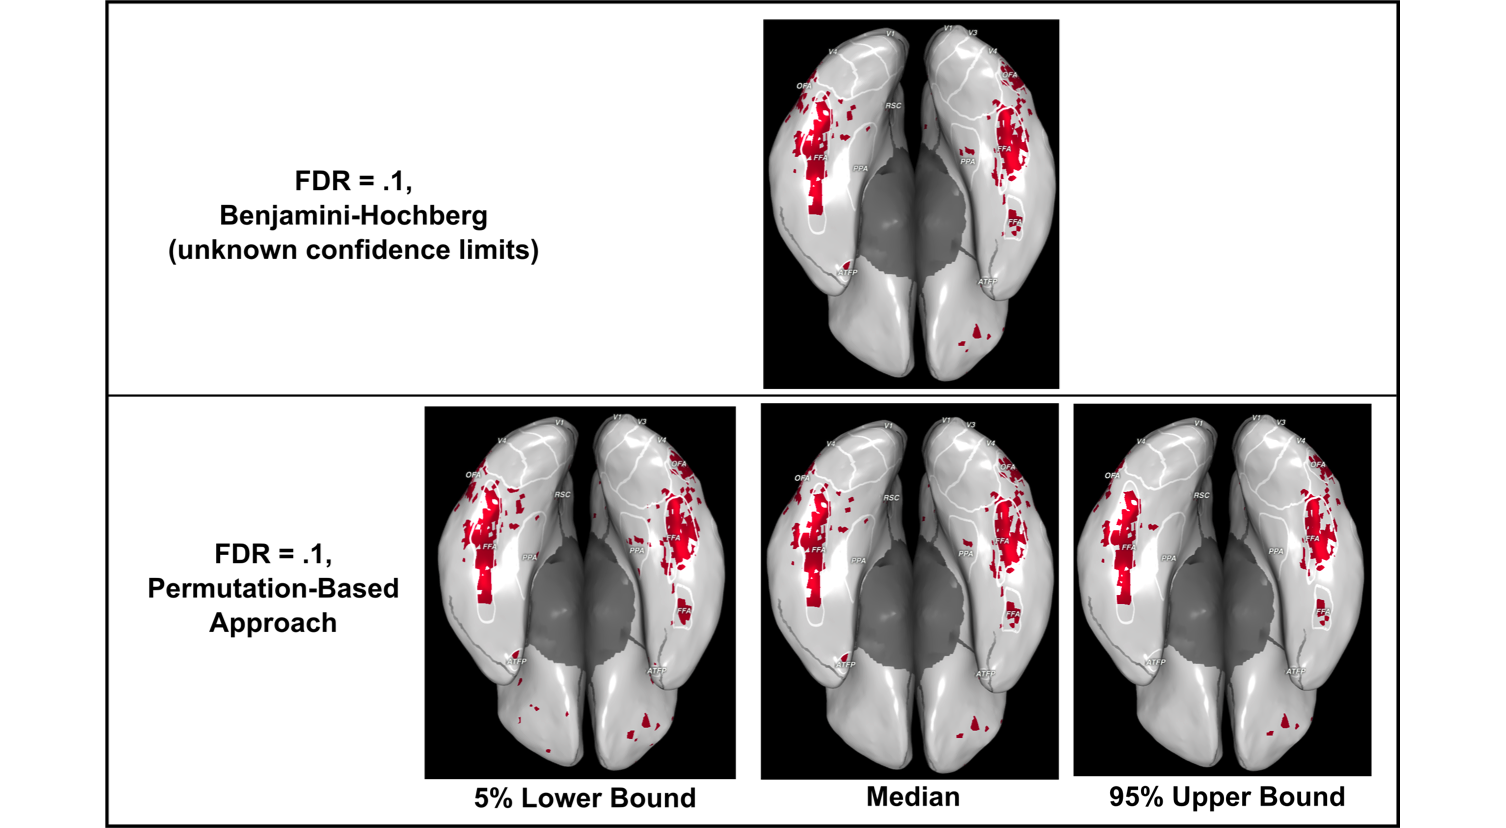
\includegraphics[scale = .70]{Figures/Slide5.png}
\caption{\footnotesize Confidence interval maps for permutation-based FDR control applied to fMRI dataset}
\end{figure}


\newpage

\section*{Part 3: Online Behavioral Testing}

This dataset comes from an online behavioral experiment that studies the perception of facial attractiveness. In this experiment, each subject was shown 40 celebrity face images and asked to give ratings for the attractiveness level of the images. The images were shown twice in two different random orders to each subject, so each image was rated twice by each subject. The dataset contains 11,600 ratings given by 145 online subjects.

Although online experiment allows cheap and fast collection of a great amount of data, it has little control on the quality of the data given by online subjects, since no experimenter is present while the subjects taking the experiment. Irresponsible subjects are a main source of this concern. In the example of this particular experiment, irresponsible subjects are referred to the subjects who do not give ratings according to the real attractiveness level of the images. They may just give the same rating to all the images, or they may just give ratings randomly in order to finish the experiment more quickly. By just calculating the variance of the ratings given by each subject, the subjects who tended to give the same rating all the time can be easily identified. However, the subjects who gave random ratings are harder to identify.

The design of this experiment allows one way of using hypothesis tests to identify the subjects who were probably giving ratings randomly. Since each subject gave two ratings to each image, if the subject was not giving ratings randomly, the correlation coefficient between his/her first ratings to each image and second ratings to each image should be reasonably higher than zero. A permutation test can quantify how significantly high a subject's correlation coefficient is. By doing a permutation test for each subject and setting up a threshold of significance level, we can maintain the subjects who are not likely to be irresponsible subjects, and exclude the others.

This method will have the multiple comparison issue described above. We can apply our permutation-based method to this example to control the false discovery rate. The procedures are discussed below. 

We set the aimed false discovery rate to 0.1. We varied the correlation coefficient threshold from 0.20 to 0.30 by steps of 0.01. The corresponding false discovery rate decreases with increasing correlation coefficient threshold (Figure 6). The most liberal threshold that satisfied our requirement was 0.23.

\begin{figure}[h c] % Centered big figure at bottom of the page ([b] argument, could be "t" for top or "h" for here)
\centering
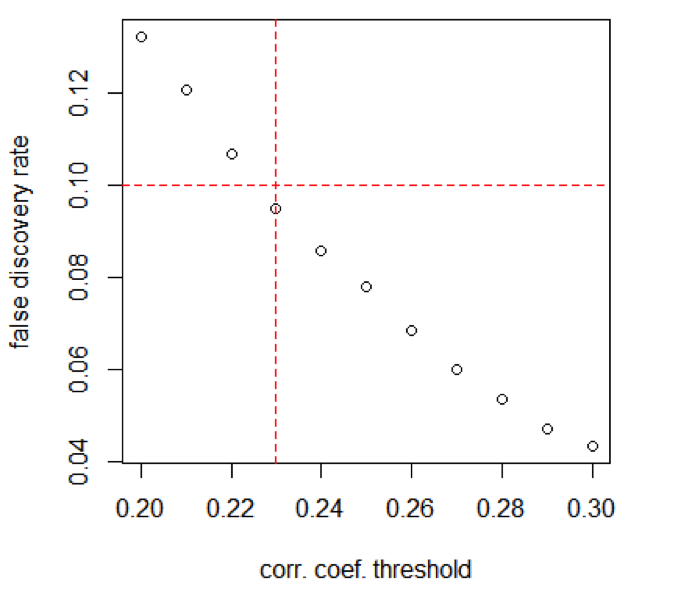
\includegraphics[scale = .70]{Figures/Part3_1.png}
\caption{\footnotesize Tested correlation coefficients and their corresponding false discovery rates. The red horizontal dashed line signifies our aimed false discovery rate. The red vertical dashed line showed the chosen correlation coefficient threshold 0.23.}
\end{figure}


The permutation simulations that were done with a threshold of 0.23 gave us the distribution of the false discovery rate when correlation threshold was set to 0.23 (Figure 7). We then calculated the 95 percent confidence interval of the false discovery rate, which was [0.05, 0.15]. Using the correlation coefficient threshold 0.23, 26 out of 145 subjects were excluded. 

\begin{figure}[h c] % Centered big figure at bottom of the page ([b] argument, could be "t" for top or "h" for here)
\centering
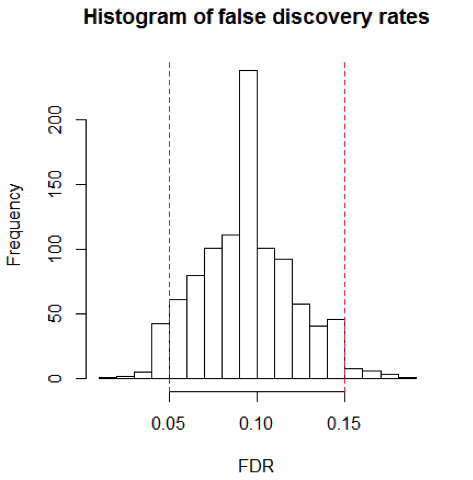
\includegraphics[scale = .90]{Figures/Part3_2.png}
\caption{\footnotesize Histogram of simulated false discovery rate when correlation coefficient threshold is 0.23. The red dashed lines signify the 95 percent confidence interval of the false discovery rate.}
\end{figure}



We compared our permutation-based method with BH method in this example. We set aimed false discovery rate to 0.1, and applied BH method to the permutation test p-values calculated for each subject, and got a p-value threshold of 0.08. The correlation coefficient of the subject whose p-value was 0.08 was 0.24, which was very close to the correlation coefficient threshold we got from our permutation-based method. Using the p-value threshold of 0.08, all the 26 subjects who were excluded by our permutation-base method were also excluded by BH method. One subject was not excluded by our permutation-based subject, but excluded by BH method (Figure 8).


In this independent tests example, our permutation-based method and BH method give very similar results, which justifies the applicability of our permutation-based method. In addition to the expected value of the false discovery rate which can also be given by BH method, our method also gives the distribution of the false discovery rate. One subject was excluded by BH method but not exclude by our permutation-based method. It is mainly because this subject has much larger permutation test p-value than the other subjects who have similar correlation coefficient with this subject. This may be due to the fact that there is little variation in this subject's ratings, so the correlation coefficient between his/her first ratings and second ratings does not change much with permutations. In fact, our permutation-based method is not limited to correlation coefficient. We can also use it to determine a permutation test p-value threshold. In that case, this method would give more coherent result with BH method. But calculating p-value threshold also requires much more computation.


\begin{figure}[h c] % Centered big figure at bottom of the page ([b] argument, could be "t" for top or "h" for here)
\centering
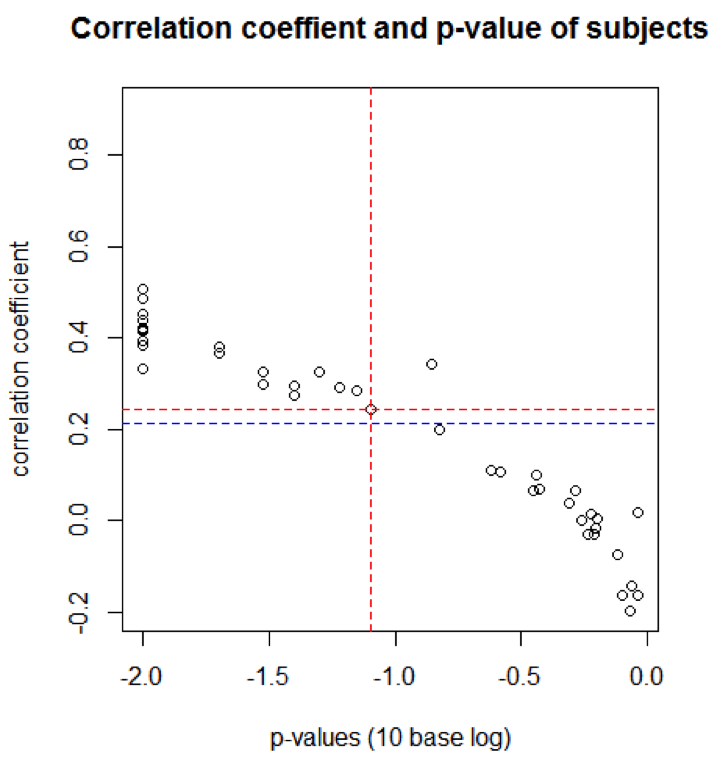
\includegraphics[scale = .70]{Figures/Part3_3.png}
\caption{\footnotesize Subjects correlation coefficient and permutation test p-values. One data point represents one subject. The blue dashed line shows the correlation coefficient threshold given by our permutation based method. The data points below the blue dashed line are the subjects excluded by our permutation based method. The vertical red dashed line shows the p-value threshold given by BH method and the horizontal red dashed line signifies the corresponding correlation coefficient. The data points to the right of the vertical red dashed line are the subjects excluded by BH method.}
\end{figure}


%----------------------------------------------------------------------------------------
%	METHODS
%----------------------------------------------------------------------------------------

\newpage

\section*{Detailed Methods}

For both part I and part II, we fit a linear model to the activity in individual voxels. Voxel activity is $ Y_{(nxq)} $, where n is the number of observations and q is the number of voxels. We predict $ Y $ using a design matrix $ X_{(nxp)} $, where p is the number of predictors, which are are either indicators of the image presentations or indicators of features contained in the images. We then estimate the coefficients using OLS (part I) or ridge regression (part II), and calculate the p-value for each coefficient in the linear model using the standard assumptions of a linear model along with normality of errors. Finally, we adjust the significance threshold for the p-values for all voxels according to either BH or permutation-based FDR control. 


\subsection*{BH}


\begin{enumerate}
  \item Set a threshold for False Discoveries (q=0.1).
 \item Sort p-values in ascending order.
 \item Iterate through p-values until p(i)<q*i/N
 \item Reject the null for tests with p-values below the ith p-value.
\end{enumerate}


\subsection*{Permutation-based FDR control}

\subsubsection*{For the simulation:}

\begin{enumerate}

\item Randomly permute the rows of the design matrix $X$.
\item Generate voxel-wise t-statistic for face > scene contrast.
\item Repeat (1-2) 1000 times to generate null distribution, in which voxel response is unrelated to whether the image is a face or a house (the label given).
\item For a range of t0 values, take average number of voxels that exceed t0 across permutation iterations. This is the expected number of false discoveries at each threshold t0, n FD (false discoveries).
\item Choose the smallest t0 such that $ \frac{FD}{nD}$ is less than q = .1, the value to which we want to control FDR. nD is the observed number of voxels with t-values above t0. 
\item To get confidence bounds, repeat 4-5, but take the 5th or 95th percentile instead of the average. 

\end{enumerate}

\subsubsection*{For the fMRI dataset:}

\begin{enumerate}
\item Randomly permute the order of images shown. Recreate the design matrix (see Figure 4).
\item Generate voxel-wise prediction correlations.
\item Repeat (1-2) 1000 times to generate null distribution, in which voxel response is unrelated to the images shown.
\item For a range of r0 values, take average number of voxels that exceed r0 across permutation iterations. This is the expected number of false discoveries at each threshold r0, n FD.
\item Choose the smallest r0 such that $ \frac{nFD}{nD}$ is less than q = .1, the value to which we want to control FDR. nD is the observed number of voxels with r-values above r0. 
\item To get confidence bounds, repeat 4-5, but take the 5th or 95th percentile instead of the average. 

\end{enumerate}

\subsubsection*{For the behavioral dataset:}

\begin{enumerate}
	\item For each subject, calculate the correlation coefficient between his/her first ratings and second ratings.
	\item Preset a threshold of correlation coefficient, and calculate the number of subjects whose correlation coefficient is higher than the threshold, denoted as m.
	\item Shuffle the second ratings of each subject.
	
	\item Compute the correlation coefficient for each subject again, and calculate how many correlation coefficients are higher than the preset threshold, denoted as $ n_1 $. This is the number of false discovery for this permutation simulation.
	
	\item Repeat procedure 3 and 4 many times, and get a series of $ n_i $. The expected false discovery rate $ q=\frac{mean(n_i)}{m} $, and the variance of the false discovery rate is $\frac{Var(n_i)}{m^2} $ .
	\item Choose another threshold of correlation coefficient and repeat procedure 2-6. Finally choose the most liberal threshold whose corresponding false discovery rate is not higher than the aimed level.
	
\end{enumerate}





%----------------------------------------------------------------------------------------
%	BIBLIOGRAPHY
%----------------------------------------------------------------------------------------


%----------------------------------------------------------------------------------------

\end{document}